\chapter{Computations (Attribute Evaluation Statements)}\indexmain{computations}\indexmain{functions}\indexmain{procedures}\indexmain{attribute evaluation}
\label{cha:computations}

In this chapter we'll have a look at the \emph{statements} of the \emph{computations} available in the rule language.
The \emph{computations} are the superordinate concept, they consist of side-effect free \emph{expressions} already introduced in \ref{cha:typeexpr}, and side-effect causing \emph{statements}.
Their corresponding abstractions are the \emph{functions} free of externally visible side-effects, defining an expression drop-in replacement, and the \emph{procedures} that can only be employed from statement context, defining a statement drop-in replacement; we'll visit those abstractions at the end of this chapter.

The most important statement is the \emph{attribute assignment}, which is used for assigning new values computed from expressions to graph element attributes.
Besides this, further types of assignments are available, and several control flow constructs as known from imperative programming languages of the C-family.
Furthermore, container methods may be called (more on this in the following chapter \ref{cha:container}), 
and global graph functions may be called (more on this in the following chapter \ref{cha:graph}).

An example implementing \indexed{depth-first search}, \indexed{breadth-first search}, and \indexed{iterative deepening} as computations of the rule language can be found in \texttt{test/should\_pass}, in \texttt{/DfsBfsSearch.grg}; you may have a look at the \verb#/computations_*.grg# files in that folder for further (but fabricated) examples.

\begin{rail}
  Statement:
      Assignment
    | CompoundAssignment
    | IndexedAssignment
    | VisitedAssignment
    | LocalVariableDecl
    | MethodCall
    | ProcedureCall
    | EmbeddedExec
    | Decision
    | Repetition
    | ForLoop
    | EarlyExit
    | ReturnStatement
    ;
\end{rail}\ixnterm{Statement}\label{computationstatemet}

%explain method calls, function calls, compound assignment, for loops in the container and graph chapters.
%The \emph{Assignment} will be explained below, the \emph{CompoundAssignment}, \emph{VisitedAssignment} and \emph{ContainerMethodCall} clauses will be introduced in chapter \ref{cha:container} and \ref{cha:graph}.


%%%%%%%%%%%%%%%%%%%%%%%%%%%%%%%%%%%%%%%%%%%%%%%%%%%%%%%%%%%%%%%%%%%%%%%%%%%%%%%%%%%%%%%%%%%%%%%%
\section{Assignments} \label{sub:assignments}\indexmain{assignments}

\begin{rail}
  Assignment:
	  NodeOrEdge '.' Ident '=' Expression ';' |
	  '::' GlobalVarIdent '.' Ident '=' Expression ';' |
	  Variable '=' Expression ';' |
	  '::' GlobalVarIdent '=' Expression ';'
	;
\end{rail}\indexmain{attribute evaluation}\ixnterm{Assignment}

Evaluation statements have \indexedsee{imperative}{attribute evaluation} semantics.
In particular, \GrG\ does not care about data dependencies (You must care for them! The assignments are just executed one after the other.).
Assignment is carried out using value semantics, even for entities of container or \texttt{string} type.
The only exception is the type \texttt{object}, there reference semantics is used.
You can find out about the available \emph{Expression}s in chapter \ref{cha:typeexpr}.

%compound assignments are given in following chapters

%%%%%%%%%%%%%%%%%%%%%%%%%%%%%%%%%%%%%%%%%%%%%%%%%%%%%%%%%%%%%%%%%%%%%%%%%%%%%%%%%%%%%%%%%%%%%%%%
\section{Local Variable Declarations} 

\begin{rail} 
  LocalVariableDecl: 
	'def' Name ':' Type ('=' Expression)? ';' |
	'def' '-' Name ':' Type '->' ('=' Expression)? ';' |
	'def' 'var' Name ':' Type ('=' Expression)? ';' |
	'def' 'ref' Name ':' Type ('=' Expression)? ';'
	;
\end{rail}\ixnterm{LocalVariableDecl}

Local variables can be defined with the syntax known for local def pattern variables, as already introduced in \ref{sec:localvarorderedevalyield}, i.e. \texttt{def var name:type} for elementary variables, or \texttt{def ref name:type} for container variables, or \texttt{def name:type} for nodes, or \texttt{def -name:type->} for edges.
At their definition, an initializing expression may be given.

\begin{example}
The following rule eval part gives some example statements regarding data flow.
  \begin{grgen}
var ::v:int;
	
rule example
{
  n:N; // we assume attributes a:int, arr:array<int>, narr:array<N>
	
	modify {
		eval {
			def var sum:int = 0; // declares a local variable of type int and initializes it
			n.a = 42; // assigns 42 to the attribute a of the node n of type N
			::v = n.a - 1; // assigns the global variable the value 41
			def ref arr:array<int> = array<int>[ sum,1,2,3 ];
			arr[0] = arr[1] + n.arr[sum];
			def ref narr:array<N> = array<N>[ n ];
			//narr[0].a = 0xAFFE; -- currently not possible, you must work around it this way:
			def tmp:N = narr[0];
			tmp.a = 0xAFFE;
			n.narr[0] = n; // this is possible in contrast
		}
	}
}
  \end{grgen}
\end{example}


%%%%%%%%%%%%%%%%%%%%%%%%%%%%%%%%%%%%%%%%%%%%%%%%%%%%%%%%%%%%%%%%%%%%%%%%%%%%%%%%%%%%%%%%%%%%%%%%
\section{Control flow} \label{sub:controlflow}\indexmain{controlflow}

Based on the value of a boolean expression different computations can be executed conditionally with the \texttt{if} and \texttt{else} statements. 
Please not that the braces are mandatory.
With the \texttt{switch} and \texttt{case} statements, you can match constants against the value of an expression computed once.
Every case-branch is enclosed in an block, at block end also the execution of the block ends,
there is no implicit fall-through carried out, a fall-through is not even available.
Only one else branch is allowed, it is hit in case no other branch was executed.
The construct is only available for expressions with values of type \texttt{byte}, \texttt{short}, \texttt{int}, \texttt{long}, \texttt{string}, \texttt{boolean}, and \texttt{enum} types.

\begin{rail} 
  Decision: IfElse | SwitchCase;
  IfElse: IfPart ((ElseIfPart)*()) (ElsePart)? ;
	IfPart: 'if' '(' BoolExpr ')' lbrace (Statement*) rbrace ;
	ElseIfPart: 'else' 'if' '(' BoolExpr ')' lbrace (Statement*) rbrace ;
	ElsePart: 'else' lbrace (Statement*) rbrace ;
	SwitchCase: 'switch' '(' Expr ')' lbrace (CaseStatement+) rbrace;
	CaseStatement: 'case' ConstExpr lbrace (Statement*) rbrace | 'else' lbrace (Statement*) rbrace;
\end{rail}\ixnterm{Decision}\ixnterm{IfElse}\ixnterm{SwitchCase}\ixkeyw{if}\ixkeyw{else}\ixkeyw{switch}\ixkeyw{case}

Computations may be executed repeatedly by the \texttt{while} and \texttt{do-while} statements. Please note that the braces are mandatory and that the \texttt{do-while} loop comes without a terminating semicolon.

\begin{rail} 
  Repetition: WhileLoop | DoWhileLoop;
	WhileLoop: 'while' '(' BoolExpr ')' lbrace (Statement*) rbrace;
	DoWhileLoop: 'do' lbrace (Statement*) rbrace 'while' '(' BoolExpr ')';
\end{rail}\ixnterm{Repetition}\ixnterm{WhileLoop}\ixnterm{DoWhileLoop}\ixkeyw{while}\ixkeyw{do}

%\section{Container iteration}

The containers introduced in chapter \ref{cha:container} may be iterated over with a for loop, one assigning the current value to a variable, the other assigning the current index and the current value to a variable.
Furthermore, a for loop is available for iterating a range of integers, with the lower and the upper bounds specified.
Moreover, a for loop is available for iterating the graph elements stored in an index, with the lower and upper bounds specified, see \ref{sub:indexusage} for more on this and the \emph{ForIndexAccessHeader}.
\begin{rail}
  ForLoop: (ForHeader | IndexedForHeader | ForRangeHeader | ForIndexAccessHeader) lbrace (Statement*) rbrace;
  ForHeader: 'for' '(' Var ':' Type 'in' ContainerVar ')';
  IndexedForHeader: 'for' '(' IndexVar ':' Type '->' Var ':' Type 'in' ContainerVar ')' ;
  ForRangeHeader: 'for' '(' Var ':' 'int' 'in' '[' IntExpr ':' IntExpr ']' ')';
\end{rail}\ixkeyw{in}\ixkeyw{for}\ixnterm{ForLoop}

Loop body execution may be exited early or continued with the next iteration with the \texttt{break} and \texttt{continue} statements. Such a statement must not occur outside of a loop.

\begin{rail} 
  EarlyExit: 
	'break' ';' |	'continue' ';'
	;
\end{rail}\ixnterm{EarlyExit}\ixkeyw{break}\ixkeyw{continue}

\begin{example}
The following rule eval part gives some example statements regarding control flow.
  \begin{grgen}
rule example
{
  n:N; // we (again) assume attributes a:int, arr:array<int>, narr:array<N>
	
	modify {
		eval {
			if(n.a < 42) {
				while(true) {
					n.a = n.a + 1;
					if(n.a == 42) {
						break; // leaves the while loop, n.a==42 afterwards
					}
				}
			} else {
				def ref narr:array<N> = n.narr;
				def var i:int = 0;
				for(tn:N in narr) {
					i = i + 1;
					n.a = n.a + tn.a + n.arr[i];
				}
			}
		}
	}
}
  \end{grgen}
\end{example}


%%%%%%%%%%%%%%%%%%%%%%%%%%%%%%%%%%%%%%%%%%%%%%%%%%%%%%%%%%%%%%%%%%%%%%%%%%%%%%%%%%%%%%%%%%%%%%%%
\section{Embedded Exec} 

As in the rules (cf. chapter \ref{cha:imperativeandstate}), \texttt{exec} statements may be embedded.
They are executing the graph rewrite sequence (see chapter \ref{cha:xgrs}) contained, with access to the variables defined outside.
This means for one reading this variables, but for the other assigning to that variables with \texttt{yield}.
The embedded \texttt{exec}s allow to apply rules from the computations, more exactly: from the procedures (embedded execs are not available in functions), while the sequence computations (cf. \ref{sec:seqcomp}) may call defined computations (functions in expression context, and procedures in statement context), mixing and merging declarative rule-based graph rewriting (pattern matching and dependent modifications) with traditional graph programming.
This construct achieves a further step in the direction of blending rule-based with traditional programming; the main step is the extension of the attribute assignments, the only statement available in the original {\scshape GrGen}, into the full-fledged computations pictured in this and the following chapters.

\begin{description}
\item[\texttt{exec(.)}] executes the graph rewrite sequence given. 
\end{description}



%%%%%%%%%%%%%%%%%%%%%%%%%%%%%%%%%%%%%%%%%%%%%%%%%%%%%%%%%%%%%%%%%%%%%%%%%%%%%%%%%%%%%%%%%%%%%%%%
\section{Computation Definition and Call} \label{sub:compdef}\indexmain{computation definition}

Computations that are occurring frequently may be factored out into a computation definition given in the header of a rule file.
Such compound computations can be built and abstracted into reusable entities in two different forms, \emph{functions} usable(/callable) from expression context, and \emph{procedures} usable(/callable) from statement context.
Besides, several built-in functions and procedures are available, ready to be called and reused with the same syntax.
(Furthermore, external functions and procedures may be declared, callable with the same syntax, too.)

%-----------------------------------------------------------------------------------------------
\subsection{Function Definition and Call}\label{sub:functions}\label{sec:funccall} 

Functions return exactly one output value, and can thus be used from the expressions with their compositional semantics.
They are side-effect free, meaning they are not allowed to change the graph while being executed ---
so you are not allowed to call procedures (self-defined as well as built-in) from with a function definition.
On the other hand do we consider pure functional programming not a help but a burden, so you are free to declare local variables and assign them as you like inside the function definitions; they only must behave as functions at the outside.

\begin{rail} 
  FunctionDefinition: 
	'function' Name '(' Parameters ')' ':' ReturnType \\
	lbrace (Statement+) rbrace;
  Parameters: (Parameter * ',');
  Parameter: IdentDecl ':' NodeType |
  '-' IdentDecl ':' EdgeType '->' |
  ('var' | 'ref') IdentDecl ':' VarType;
\end{rail}\ixnterm{FunctionDefinition}\ixnterm{Parameter}\ixkeyw{function}\ixkeyw{var}\ixkeyw{ref}

The function definition must return a value with a return statement (so there must be at least one return statement).
The type of the one return value must be compatible to the return type specified in the computation definition.
(A return statement must not occur outside of a computation definition.)

\begin{rail}
  ReturnStatement: 'return' '(' Expression ')' ';' ;
\end{rail}\ixkeyw{return}\ixnterm{ReturnStatement}

\begin{rail}
  FunctionCall: Name '(' (Expression * ',') ')' ;
\end{rail}\ixnterm{FunctionCall}

\begin{example}
An example showing how functions are declared and used.
  \begin{grgen}
function fac(var x:int) : int
{
	if(x>1) {
		return( x * fac(x-1) );
	} else {
		return( 1 );
	}
}
function foo(m:N) : boolean
{
	def var tmp:int = fac(m.a);
	tmp = tmp - 1;
	return( m.a < tmp );
}
test example : (int)
{
	n:N;
	if{foo(n);}
	return ( fac(n.a) );
}
  \end{grgen}
\end{example}

A such defined function may then be called as an expression atom from anywhere in the rule language file where an expression is required; or even from the sequence computations where an expression is required.
Besides the built-in functions that are called with the same syntax;
table~\ref{funcstab} and table~\ref{funcstab2} list the global built-in functions of the rule language at a glance,
table~\ref{packagefuncstab} lists the built-in functions contained in built-in packages at a glance.

%\makeatletter
\begin{table}[htbp]
\centering
\begin{tabular}{|l|}
\hline
\texttt{nodes([NodeType]):set<Node>}\\
\texttt{edges([EdgeType]):set<Edge>}\\
\hline
\texttt{source(Edge):Node}\\
\texttt{target(Edge):Node}\\
\texttt{opposite(Edge,Node):Node}\\
\hline
\texttt{adjacent(Node[,EdgeType[,NodeType]]):set<Node>}\\
\texttt{adjacentIncoming(Node[,EdgeType[,NodeType]]):set<Node>}\\
\texttt{adjacentOutgoing(Node[,EdgeType[,NodeType]]):set<Node>}\\
\texttt{incident(Node[,EdgeType[,NodeType]]):set<Edge>}\\
\texttt{incoming(Node[,EdgeType[,NodeType]]):set<Edge>}\\
\texttt{outgoing(Node[,EdgeType[,NodeType]]):set<Edge>}\\
\hline
\texttt{reachable(Node[,EdgeType[,NodeType]]):set<Node>}\\
\texttt{reachableIncoming(Node[,EdgeType[,NodeType]]):set<Node>}\\
\texttt{reachableOutgoing(Node[,EdgeType[,NodeType]]):set<Node>}\\
\texttt{reachableEdges(Node[,EdgeType[,NodeType]]):set<Edge>}\\
\texttt{reachableEdgesIncoming(Node[,EdgeType[,NodeType]]):set<Edge>}\\
\texttt{reachableEdgesOutgoing(Node[,EdgeType[,NodeType]]):set<Edge>}\\
\hline
\texttt{boundedReachable(Node,int[,EdgeType[,NodeType]]):set<Node>}\\
\texttt{boundedReachableIncoming(Node,int[,EdgeType[,NodeType]]):set<Node>}\\
\texttt{boundedReachableOutgoing(Node,int[,EdgeType[,NodeType]]):set<Node>}\\
\texttt{boundedReachableEdges(Node,int[,EdgeType[,NodeType]]):set<Edge>}\\
\texttt{boundedReachableEdgesIncoming(Node,int[,EdgeType[,NodeType]]):set<Edge>}\\
\texttt{boundedReachableEdgesOutgoing(Node,int[,EdgeType[,NodeType]]):set<Edge>}\\
\hline
\texttt{boundedReachableWithRemainingDepth(Node,int):map<Node, int>}\\
\texttt{boundedReachableWithRemainingDepthIncoming(Node,int):map<Node, int>}\\
\texttt{boundedReachableWithRemainingDepthOutgoing(Node,int):map<Node, int>}\\
The three functions above allow optional edge and node type constraints, too.\\
\hline
\texttt{inducedSubgraph(set<Node>):graph}\\
\texttt{definedSubgraph(set<Edge>):graph}\\
\texttt{equalsAny(graph, set<graph>):boolean}\\
\texttt{equalsAnyStructurally(graph, set<graph>):boolean}\\
\texttt{copy(graph):graph}\\
\texttt{copy(container):container}\\
\texttt{copy(match<r>):match<r>}\\
\hline
\texttt{random():double}\\
\texttt{random(int):int}\\
\hline
\texttt{nameof(Node/Edge/graph):string}\\
\texttt{uniqueof(Node/Edge/graph):int}\\
\texttt{nodeByName(string):Node}\\
\texttt{edgeByName(string):Edge}\\
\texttt{nodeByUnique(int):Node}\\
\texttt{edgeByUnique(int):Edge}\\
\hline
\end{tabular}
\caption{Global functions at a glance, part I}
\label{funcstab}
\end{table}

%\makeatletter
\begin{table}[htbp]
\centering
\begin{tabular}{|l|}
\hline
\texttt{countNodes([NodeType]):int}\\
\texttt{countEdges([EdgeType]):int}\\
\hline
\texttt{countAdjacent(Node[,EdgeType[,NodeType]]):int}\\
\texttt{countAdjacentIncoming(Node[,EdgeType[,NodeType]]):int}\\
\texttt{countAdjacentOutgoing(Node[,EdgeType[,NodeType]]):int}\\
\texttt{countIncident(Node[,EdgeType[,NodeType]]):int}\\
\texttt{countIncoming(Node[,EdgeType[,NodeType]]):int}\\
\texttt{countOutgoing(Node[,EdgeType[,NodeType]]):int}\\
\hline
\texttt{countReachable(Node[,EdgeType[,NodeType]]):int}\\
\texttt{countReachableIncoming(Node[,EdgeType[,NodeType]]):int}\\
\texttt{countReachableOutgoing(Node[,EdgeType[,NodeType]]):int}\\
\texttt{countReachableEdges(Node[,EdgeType[,NodeType]]):int}\\
\texttt{countReachableEdgesIncoming(Node[,EdgeType[,NodeType]]):int}\\
\texttt{countReachableEdgesOutgoing(Node[,EdgeType[,NodeType]]):int}\\
\hline
\texttt{countBoundedReachable(Node,int[,EdgeType[,NodeType]]):int}\\
\texttt{countBoundedReachableIncoming(Node,int[,EdgeType[,NodeType]]):int}\\
\texttt{countBoundedReachableOutgoing(Node,int[,EdgeType[,NodeType]]):int}\\
\texttt{countBoundedReachableEdges(Node,int[,EdgeType[,NodeType]]):int}\\
\texttt{countBoundedReachableEdgesIncoming(Node,int[,EdgeType[,NodeType]]):int}\\
\texttt{countBoundedReachableEdgesOutgoing(Node,int[,EdgeType[,NodeType]]):int}\\
\hline
\texttt{isAdjacent(Node,Node[,EdgeType[,NodeType]]):boolean}\\
\texttt{isAdjacentIncoming(Node,Node[,EdgeType[,NodeType]]):boolean}\\
\texttt{isAdjacentOutgoing(Node,Node[,EdgeType[,NodeType]]):boolean}\\
\texttt{isIncident(Node,Edge[,EdgeType[,NodeType]]):boolean}\\
\texttt{isIncoming(Node,Edge[,EdgeType[,NodeType]]):boolean}\\
\texttt{isOutgoing(Node,Edge[,EdgeType[,NodeType]]):boolean}\\
\hline
\texttt{isReachable(Node,Node[,EdgeType[,NodeType]]):boolean}\\
\texttt{isReachableIncoming(Node,Node[,EdgeType[,NodeType]]):boolean}\\
\texttt{isReachableOutgoing(Node,Node[,EdgeType[,NodeType]]):boolean}\\
\texttt{isReachableEdges(Node,Edge[,EdgeType[,NodeType]]):boolean}\\
\texttt{isReachableEdgesIncoming(Node,Edge[,EdgeType[,NodeType]]):boolean}\\
\texttt{isReachableEdgesOutgoing(Node,Edge[,EdgeType[,NodeType]]):boolean}\\
\hline
\texttt{isBoundedReachable(Node,Node,int[,EdgeType[,NodeType]]):boolean}\\
\texttt{isBoundedReachableIncoming(Node,Node,int[,EdgeType[,NodeType]]):boolean}\\
\texttt{isBoundedReachableOutgoing(Node,Node,int[,EdgeType[,NodeType]]):boolean}\\
\texttt{isBoundedReachableEdges(Node,Edge,int[,EdgeType[,NodeType]]):boolean}\\
\texttt{isBoundedReachableEdgesIncoming(Node,Edge,int[,EdgeType[,NodeType]]):boolean}\\
\texttt{isBoundedReachableEdgesOutgoing(Node,Edge,int[,EdgeType[,NodeType]]):boolean}\\
\hline
\end{tabular}
\caption{Global functions at a glance, part II}
\label{funcstab2}
\end{table}

\begin{table}[htbp]
\centering
\begin{tabular}{|l|}
\hline
\texttt{Math::min(Number,Number):Number}\\
\texttt{Math::max(Number,Number):Number}\\
\texttt{Math::abs(Number):Number}\\
\hline
\texttt{Math::ceil(double):double}\\
\texttt{Math::floor(double):double}\\
\texttt{Math::round(double):double}\\
\texttt{Math::truncate(double):double}\\
\hline
\texttt{Math::pow([double,]double):double}\\
\texttt{Math::log(double[,double]):double}\\
\texttt{Math::sgn(double):double}\\
\hline
\texttt{Math::sin(double):double}\\
\texttt{Math::cos(double):double}\\
\texttt{Math::tan(double):double}\\
\hline
\texttt{Math::arcsin(double):double}\\
\texttt{Math::arccos(double):double}\\
\texttt{Math::arctan(double):double}\\
\hline
\texttt{Math::pi():double}\\
\texttt{Math::e():double}\\
\hline
\texttt{Math::byteMin():byte}\\
\texttt{Math::byteMax():byte}\\
\texttt{Math::shortMin():short}\\
\texttt{Math::shortMax():short}\\
\texttt{Math::intMin():int}\\
\texttt{Math::intMax():int}\\
\texttt{Math::longMin():long}\\
\texttt{Math::longMax():long}\\
\texttt{Math::floatMin():float}\\
\texttt{Math::floatMax():float}\\
\texttt{Math::doubleMin():double}\\
\texttt{Math::doubleMax():double}\\
\hline
\texttt{File::import(string):graph}\\
\texttt{File::exists(string):boolean}\\
\hline
\texttt{Time::now():long}\\
\hline
\end{tabular}
\caption{Functions in packages at a glance}
\label{packagefuncstab}
\end{table}


%-----------------------------------------------------------------------------------------------
\subsection{Procedure Definition And Call}\label{sub:procedures}\label{sec:proccall} 
%You may call any of the built-in procedures that will be introduced in the following chapters or any of your defined procedures just for its side effects, throwing away the result.

Procedures may return between zero and $k$ (arbitrary, but statically fixed) output values, and are thus only callable as a statement, with (or without) a multiple-value assignment.
They are allowed to manipulate the graph as needed while being executed;
so in a procedure definition you are free to call other procedures (self-defined as well as built-in).

\begin{rail} 
  ProcedureDefinition: 
	'procedure' Name '(' Parameters ')' ReturnTypes \\
	lbrace (Statement+) rbrace;
  ReturnTypes: (':' '(' (ReturnType + ',') ')' )?;
\end{rail}\ixnterm{ProcedureDefinition}\ixnterm{Parameter}\ixkeyw{procedure}\ixkeyw{var}\ixkeyw{ref}

Please note the syntactic difference distinguishing the procedures from the functions (besides the different keyword): the return types are enclosed in parenthesis (or omitted altogether).
The computation definition may return between zero and $k$ values.
It must be always ended with a return statement; the type of the return values must be compatible to the return types specified in the computation definition.
(A return statement must not occur outside of a computation definition.)

\begin{rail}
  ReturnStatement: 'return' ( '(' (Expression + ',') ')' )? ';' ;
\end{rail}\ixkeyw{return}\ixnterm{ReturnStatement}

\begin{rail}
  ProcedureCall: (OutputAssignment)? Name '(' (Expression * ',') ')' ;
  OutputAssignment: '(' (AssignmentTarget + ',') ')' '=' ;
\end{rail}\ixnterm{ProcedureCall}\ixnterm{OutputAssignment}\ixnterm{AssignmentTarget}

\begin{example}
An example showing how procedures are declared and used.
  \begin{grgen}
procedure foo(n:N) : (N,int)
{
	(def m:N) = add(N); // create new node of type N and add it to the graph
	return( m, n.a );
}

procedure bar(m:N, var i:int)
{
	def var fac:int = 1;
	while(i>0) {
		fac = fac * i;
		i = i - 1;
	}
	m.a = m.a - fac;
	return;
}

rule example : (int,int)
{
	n:N;
	modify {
		def var i:int;
		eval {
			def m:N;
			(m,yield i)=foo(n);
			bar(m,i);
		}
		return(i,n.a);
	}
}
  \end{grgen}
\end{example}

A such defined procedure may then be called as a statement atom from anywhere in the rule language file where an attribute evaluation (/computation) is required; or even from the sequence computations where a statement is required.
Besides the built-in procedures that are called with the same syntax;
table~\ref{procstab} lists the global built-in procedures of the rule language at a glance,
table~\ref{packageprocstab} lists the built-in procedures contained in built-in packages at a glance.

Please note that the \emph{OutputAssignment} is optional, you may execute a procedure just for its side effects; this kind of call is even the most common as many built-in procedures don't return values at all but are just executed for their state changes.
The \emph{AssignmentTarget} may be any of the LHS expressions supported by the different \emph{AssignmentStatements} (a def variable, a def variable yielded to, a global variable, a graph element attribute, an indexed target, or a visited flag of a graph element), and it may be def variable that gets just declared (\emph{LocalVariableDecl}), using the procedure output for initialization.

%\makeatletter
\begin{table}[htbp]
\centering
\begin{tabular}{|l|}
\hline
\texttt{add(NodeType):(Node)}\\
\texttt{addCopy(Node):(Node)}\\
\texttt{add(EdgeType,Node,Node):(Edge)}\\
\texttt{addCopy(Edge,Node,Node):(Edge)}\\
\texttt{rem(Node)}\\
\texttt{rem(Edge)}\\
\texttt{retype(Node,NodeType):(Node)}\\
\texttt{retype(Edge,EdgeType):(Edge)}\\
\texttt{clear()}\\
\hline
\texttt{merge(Node,Node)}\\
\texttt{redirectSource(Edge,Node)}\\
\texttt{redirectTarget(Edge,Node)}\\
\texttt{redirectSourceAndTarget(Edge,Node,Node)}\\
\hline
\texttt{insert(graph)}\\
\texttt{insertCopy(graph,Node):(Node)}\\
\texttt{insertInduced(set<Node>,Node):(Node)}\\
\texttt{insertDefined(set<Edge>,Edge):(Edge)}\\
\hline
\texttt{valloc():(int)}\\
\texttt{vfree(int)}\\
\texttt{vreset(int)}\\
\texttt{vfreenonreset(int)}\\
\hline
\texttt{emit(string(,string)*)}\\
\texttt{record(string)}\\
\hline
\end{tabular}
\caption{Global procedures at a glance}
\label{procstab}
\end{table}

%\makeatletter
\begin{table}[htbp]
\centering
\begin{tabular}{|l|}
\hline
\texttt{File::export(string)}\\
\texttt{File::export(graph,string)}\\
\texttt{File::delete(string)}\\
\hline
\texttt{Transaction::start():(int)}\\
\texttt{Transaction::pause(int)}\\
\texttt{Transaction::resume(int)}\\
\texttt{Transaction::commit(int)}\\
\texttt{Transaction::rollback(int)}\\
\hline
\texttt{Debug::add(string(,object)*)}\\
\texttt{Debug::rem(string(,object)*)}\\
\texttt{Debug::emit(string(,object)*)}\\
\texttt{Debug::halt(string(,object)*)}\\
\texttt{Debug::highlight(string(,object,string)*)}\\
\hline
\end{tabular}
\caption{Procedures in packages at a glance}
\label{packageprocstab}
\end{table}

\pagebreak

%%%%%%%%%%%%%%%%%%%%%%%%%%%%%%%%%%%%%%%%%%%%%%%%%%%%%%%%%%%%%%%%%%%%%%%%%%%%%%%%%%%%%%%%%%%%%%%%
\section{The Big Picture}
Figure \ref{figcomptypescallsuses} displays the different computation types of \GrG, and how they may use and call each other. On top the strategy language for rule control, to the left the declarative rules and subpatterns, and to the right the imperative parts for attribute computations or traditional graph programming. The statements include the expressions and non-graph changing statements.

\begin{figure}[hptb]
  \centering
  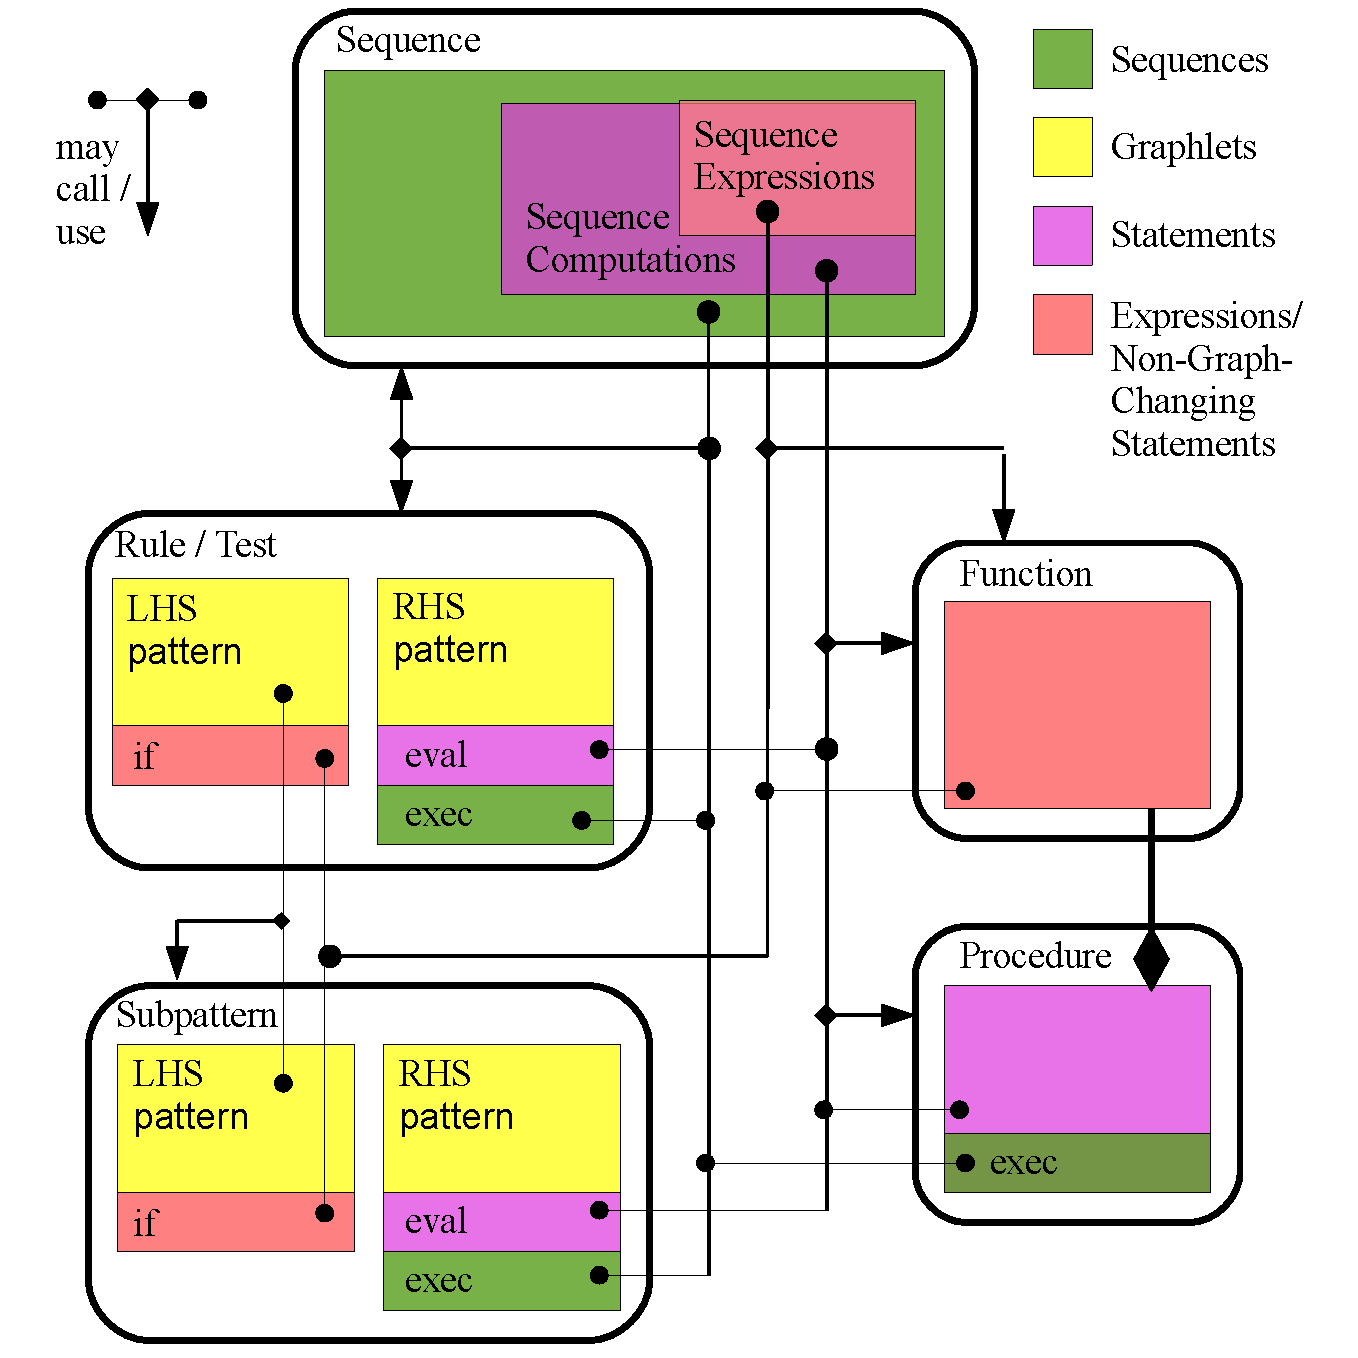
\includegraphics[width=1.0\textwidth]{fig/ComputationContainmentAndCallability}
  \caption{Computation Types and Possible Calls/Uses}
  \label{figcomptypescallsuses}
\end{figure}

The following tables give an overview over the rule and computation sublanguages of \GrG;
separated into pattern and rewrite part, and into expressions and statements.

 %\makeatletter
\begin{table}[htbp]
\begin{minipage}{\linewidth} \renewcommand{\footnoterule}{} 
\begin{tabularx}{\linewidth}{|lX|}
\hline
\texttt{.}	& Declaration of an anonymous node of type \texttt{Node}, to be matched. \\
\texttt{-->}	& Declaration of an anonymous edge of type \texttt{Edge}, to be matched. \\
\texttt{<-->}	& Declaration of an anonymous edge of type \texttt{Edge} that can get matched in either direction. \\
\texttt{--}	& Declaration of an anonymous undirected edge of type \texttt{UEdge}, to be matched. \\
\texttt{n:N} & Declaration of a node \texttt{n} of type \texttt{N}, to be matched.\\
\texttt{-e:E->} & Declaration of an edge \texttt{e} of type \texttt{E}, to be matched.\\
\texttt{n} & Reference to node \texttt{n} within a graphlet.\\
\texttt{-e->} & Reference to edge \texttt{e} within a graphlet.\\
\texttt{def var v:B}	& Defines a def-variable \texttt{v} of basic type \texttt{B}, to be yielded to.\\
\texttt{def ref c:C}	& Defines a def-variable \texttt{c} of container type \texttt{C}, to be yielded to.\\
\hline
\texttt{x:typeof(y)} & The element \texttt{x} to be matched must be of the same or a subtype as \texttt{y}.\\
\texttt{x:T{\textbackslash}S} & The element \texttt{x} must be of type \texttt{T} but not of subtype \texttt{S}.\\
\texttt{x:T<y>} & The element \texttt{y} casted to \texttt{T}, accessible as \texttt{x}.\\
\hline
\texttt{hom(x,y)} & The pattern elements \texttt{x} and \texttt{y} are allowed to match the same graph element.\\
\texttt{independent(x)} & The pattern element \texttt{x} may be matched homomorphically to all other pattern elements.\\
\texttt{exact(x,y)} & All edges incident to \texttt{x} and \texttt{y} in the host graph must have been specified in the pattern.\\
\texttt{induced(x,y)} & Induced edges in between \texttt{x} and \texttt{y} in the host graph must have been specified in the pattern.\\
\hline
\texttt{if\{exp;\}} & An attribute condition constraining the pattern.\\
\texttt{yield\{stmt\}} & A computation for yielding to def variables.\\
\hline
\texttt{nested\{pattern\}} & A nested pattern, with \texttt{nested} being one of the pattern construction modi listed in \ref{keywordregexpsyntax}.\\
\hline
\texttt{p:P()} & A usage/call \texttt{p} of a (user-defined) subpattern of type \texttt{P}.\\
\hline
\end{tabularx}
\end{minipage}\\
\\ 
{\small Let \texttt{exp} be an expression, \texttt{stmt} be a statement, and \texttt{pattern} be a LHS pattern.}
\caption{Pattern (LHS) elements at a glance}
\label{patternstab}
\end{table}
%\makeatother

 %\makeatletter
\begin{table}[htbp]
\begin{minipage}{\linewidth} \renewcommand{\footnoterule}{} 
\begin{tabularx}{\linewidth}{|lX|}
\hline
\texttt{modify\{pattern\}}	& An RHS pattern nested in an arbitrary LHS pattern, specifying the changes. \\
\texttt{replace\{pattern\}}	& An RHS pattern nested in an arbitrary LHS pattern, specifying the target pattern. \\
\hline
\texttt{.}	& Declaration of an anonymous node of type \texttt{Node}, to be created. \\
\texttt{-->}	& Declaration of an anonymous edge of type \texttt{Edge}, to be created. \\
\texttt{n:N} & Declaration of a node \texttt{n} of type \texttt{N}, to be created.\\
\texttt{-e:E->} & Declaration of an edge \texttt{e} of type \texttt{E}, to be created.\\
\texttt{n} & Reference to node \texttt{n} within a graphlet, ensures it is kept in \texttt{replace} mode.\\
\texttt{-e->} & Reference to edge \texttt{e} within a graphlet, ensures it is kept in \texttt{replace} mode.\\
\texttt{def var v:B}	& Defines a def-variable \texttt{v} of basic type \texttt{B}, to be yielded to.\\
\texttt{def ref c:C}	& Defines a def-variable \texttt{c} of container type \texttt{C}, to be yielded to.\\
\texttt{delete(x)} & Deletes element \texttt{x} in \texttt{modify} mode.\\
\hline
\texttt{x:typeof(y)} & The element \texttt{x} is created with the same type as \texttt{y}.\\
\texttt{x:T<y>} & The element \texttt{y} is casted to type \texttt{T}, accessible as \texttt{x} afterwards.\\
\texttt{x:copy<y>} & The element \texttt{x} is created as exact copy of \texttt{y}.\\
\texttt{x:typeof(y)<y,z>} & The nodes \texttt{y} and \texttt{z} are merged and casted to the original type of \texttt{y}, accessible as \texttt{x} afterwards.\\
\texttt{x !-e->! y} & The edge \texttt{e} is redirected to source node \texttt{x} and target node \texttt{y}.\\
\hline
\texttt{eval\{stmt\}} & A computation assigning to attributes or def variables.\\
\hline
\texttt{exec(s ;> yield o=i)} & Executes the sequence \texttt{s}, and then yields the value of an inner variable \texttt{i} to an outer variable \texttt{o}. Yielding from an \texttt{exec} is only possible in the top-level \texttt{exec} of a rule, in nested patterns and subpatterns the \texttt{exec}ution is deferred.\\
\hline
\texttt{delete(p)} & Deletes the subpattern used as \texttt{p}.\\
\texttt{:P()} & Creates a simple subpattern of type \texttt{P}.\\
\texttt{:p()} & Uses or calls the rewrite part of a (user-defined) subpattern used as \texttt{p} in the containing LHS pattern.\\
\hline
\end{tabularx}
\end{minipage}\\
\\ 
{\small Let \texttt{stmt} be a statement.}
\caption{Rewrite elements (RHS pattern) at a glance}
\label{rewritestab}
\end{table}
%\makeatother

%\makeatletter
\begin{table}[htbp]
\begin{minipage}{\linewidth} \renewcommand{\footnoterule}{} 
\begin{tabularx}{\linewidth}{|lX|}
\hline
\texttt{v}	& Reads the variable \texttt{v}. \\
\texttt{::v}	& Reads the global variable \texttt{v}. \\
\texttt{v.a} & Reads the attribute \texttt{a} of \texttt{v}.\\
\texttt{v[i]} & Reads the value at position \texttt{i} of container \texttt{v}.\\
\texttt{idx[n]} & Reads the incidence count of node \texttt{n} from incidence count index \texttt{idx}.\\
\texttt{x.a[i]} & Reads the value at position \texttt{i} of container attribute \texttt{a} of \texttt{x}.\\
\texttt{x.visited[i]} & Reads the visited flag \texttt{i} of graph element \texttt{x}.\\
\hline
\texttt{typeof(v)}	& Returns the type of graph element \texttt{v}. \\
\texttt{(T)v}	& Casts \texttt{v} to type \texttt{T}. \\
\texttt{nameof(v)}	& Returns the name of graph element \texttt{v}. \\
\texttt{random()}	& Returns a random value in between 0.0 and 1.0. \\
\hline
\texttt{cond ? exp1 :~exp2}	& Returns \texttt{exp1} if \texttt{cond}, otherwise \texttt{exp2}. \\
\texttt{e op f}	& For \texttt{op} being one of the binary operators listed in \ref{tabopprios}. \\
\texttt{op f}	& For \texttt{op} being one of the unary operators listed in \ref{tabopprios}. \\
\hline
\texttt{f(...)}	& Calls one of the functions listed in \ref{funcstab}. Or calls a user defined function \texttt{f}. \\
\texttt{v.fm(...)}	& Calls one of the function methods listed in \ref{funcmethstab}. Or calls a user defined function method \texttt{fm}.\\
\hline
\end{tabularx}
\end{minipage}\\
\\ 
{\small Let \texttt{cond}, \texttt{exp1}, and \texttt{exp2} be expressions.}
\caption{Expressions at a glance}
\label{expressionstab}
\end{table}
%\makeatother

 %\makeatletter
\begin{table}[htbp]
\begin{minipage}{\linewidth} \renewcommand{\footnoterule}{} 
\begin{tabularx}{\linewidth}{|lX|}
\hline
\texttt{def n:N}	& Defines a variable \texttt{n} of node type \texttt{N}.\\
\texttt{def -e:E->}	& Defines a variable \texttt{e} of edge type \texttt{E}.\\
\texttt{def var v:B}	& Defines a variable \texttt{v} of basic type \texttt{B}.\\
\texttt{def ref c:C}	& Defines a variable \texttt{c} of container type \texttt{C}.\\
\hline
\texttt{v = exp} & Assigns the value of \texttt{exp} to the variable \texttt{v}.\\
\texttt{::v = exp} & Assigns the value of \texttt{exp} to the global variable \texttt{v}.\\
\texttt{v.a = exp} & Assigns the value of \texttt{exp} to the attribute \texttt{a} of \texttt{v}.\\
\texttt{v[i] = exp} & Assigns the value of \texttt{exp} to the position \texttt{i} of container \texttt{v}.\\
\texttt{x.a[i] = exp} & Assigns the value of \texttt{exp} to the position \texttt{i} of container attribute \texttt{a} of \texttt{x}.\\
\texttt{x.visited[i] = exp} & Assigns the value of \texttt{exp} to the visited flag \texttt{i} of graph element \texttt{x}.\\
\hline
\texttt{if(cond) \{S1\} else \{S2\}} & Executes \texttt{S1} iff \texttt{cond} evaluates to \texttt{true}, or \texttt{S2} otherwise.\\
\texttt{switch(exp) \{ cases \}} & Evaluates \texttt{exp}, then dispatches to one of the cases, see below.\\
\texttt{case c-exp \{S1\} else \{S2\}} & If the \texttt{c}onstant \texttt{exp} matches the value switched upon, \texttt{S1} is executed, if none of the cases matches, \texttt{else} is executed (if given).\\
\texttt{while(cond) \{S1\} } & Executes \texttt{S1} as long as \texttt{cond} evaluates to s\texttt{true}.\\
\texttt{do \{S1\} while(cond) } & Executes \texttt{S1} until \texttt{cond} evaluates to \texttt{false}.\\
\texttt{for(v:T in c) \{S1\} } & Executes \texttt{S1} for each value \texttt{v} contained in container \texttt{c}.\\
\texttt{for(i:T->v:S in c) \{S1\} } & Executes \texttt{S1} for each key/position to value pair \texttt{(i,v)} contained in container \texttt{c}.\\
\texttt{for(i:int in [l:r]) \{S1\} } & Executes \texttt{S1} for each integer \texttt{i} in the range from \texttt{l} to \texttt{r}, in steps of 1, upwards if \texttt{l<=r}, otherwise downwards.\\
\texttt{for(n:N in \{asc.(idx>7)\}) \{S1\}}	& Execute \texttt{S1} for every \texttt{n} in the index \texttt{idx}, in ascending order, from \texttt{7} exclusive on. \texttt{asc.} abbreviates \texttt{ascending}, is not valid syntax as such.\\
\hline
\texttt{break} & Aborts execution of the containing loop.\\
\texttt{continue} & Continues execution of the containing loop at its condition.\\
\texttt{return} & Returns from a containing function or procedure.\\
\texttt{return(v)} & Returns from a containing function or procedure with result value \texttt{v}.\\
\hline
\texttt{exec(s ;> yield o=i)} & Executes the sequence \texttt{s}, and then yields the value of an inner variable \texttt{i} to an outer variable \texttt{o}.\\
\hline
\texttt{(...)=p(...)}	& Calls one of the procedures listed in \ref{procstab}. Or calls a user defined procedure \texttt{p}.\\
\texttt{(...)=v.pm(...)}	& Calls one of the procedure methods listed in \ref{procmethstab}. Or calls a user defined procedure method \texttt{pm}.\\
\hline
\texttt{exec(s)} & Executes the sequence \texttt{s}.\\
\hline
\end{tabularx}
\end{minipage}\\
\\ 
{\small Let \texttt{exp} and \texttt{cond} be expressions, and \texttt{S1} and \texttt{S2} be statements}
\caption{Statements at a glance}
\label{statementstab}
\end{table}
%\makeatother



